% !TEX root = main.tex
\chapter{Introduction}
\label{introchap}

\section{Motivation}
This thesis focuses on the implementation and development of a 6 degree-of-freedom (DoF) guidance algorithm that solves the powered descent guidance (PDG) problem. I present a modified version of the Szmuk-Açıkmeşe 6-DoF algorithm presented in \cite{szmuk2018successive}.


\subsection{Attributes of a Good Guidance Algorithm}
minimal computational complexity

accurate to the dynamics

can be recomputed online when needed

has a free final time option

incorporates important system and mission constraints

optimality of some sorts

guarantees of convergence or optimality

simple FDIR recovery

% #########################################
% Introduction basically
\section{Background}
Pin-point landing has been of significant interest in the last 6 decades for a variety of applications. These include safely landing scientific payloads and humans on other planets or back on Earth. Having the ability to land near a site of scientific interest, a base, or refueling station will become a requirement as we build our space transportation infrastructure. Solving this problem has also been of considerable interest to those returning launch vehicle stages 

The ability to soft-land a rocket is fundamentally disruptive to the launch industry and has already had a large impact in reducing the cost of getting to space. Additionally, similar methods, given navigational upgrades, will be conducive of the development of colonies on other planets. Pin-point landing and divert capability is a necessity in these situations.

Every pinpoint landing problem begins with an entry phase where the vehicle descends through an atmosphere to a point where powered descent must begin. Many Mars entry, descent, and landing schemes enter the atmosphere and slow down via parachute. This parachute is then cut away to allow powered descent. With atmospheric qualities being stochastic, the position in which the descent phase must begin is uncertain. Therefore, we would like to look at algorithms which maximize the divert capability of the craft by minimizing the fuel consumption or final time from initial condition to terminal state. We define powered descent guidance as the generation of a fuel-optimal trajectory that takes the vehicle from some initial state condition to a prescribed final state in a uniform gravitational field with standard vehicle given thrust magnitude and direction constraints.

The convex optimization framework is exploited because it is conducive of real-time on-board implementation and has guaranteed convergence properties with deterministic criteria. The convex programming algorithm to solve powered descent guidance that I will present has non-convex controls constraints and will be posed as a finite-dimensional SOCP problem. SOCPs have low complexity and can be solved in polynomial time \cite{boyd2004convex}. Interior-point numerical methods compute optimal solutions with deterministic stopping criteria and are, again conducive to on-board implementation. 



% #########################################
\section{Related Research}
perhaps start with lawden functions linear in control?

"Lossless convexification can be used to convexify non-convex constraints without losing precision,
unfortunately, only a few types of constraint can be convexified by lossless convexification. The nonlinear dynamics
and constraints are the primary factors for non-convexity in P1 and they are not in the scope of lossless
convexification. In this subsection, an improved successive convexification algorithm is proposed to circumvent the
non-convexity from nonlinearity. "

COMPARE AND CONTRAST WITH SIMILAR ONLINE MTHODS LIKE LOSSLESS CONVEXIFICAION

COMPARE AND CONTRAST FRAMEWORKW ITH SQP


\section{Brief Introduction to Convex Optimization}

\section{On Successive Convexification}

% #########################################
\section{Statement of Scope}














% BELOW THIS LINE ARE TUTORIALS ON THINGS FROM THE TEMPLATE

% \begin{figure}[htbp]
% 	\caption[Cylinder and measurements]{
% 	This diagram of a cylinder and various
% 	measurements and quantities was actually
% 	made using {\bf xfig}, a freeware
% 	drawing program for Unix systems.
% 	Diagrams can be exported directly to PDF
% 	files, the preferred format for
% 	vector graphics.  Vector graphics can
% 	be magnified indefinitely without degradation,
% 	whereas bitmap images (JPG and PNG)
% 	must be pretty high-resolution if you don't
% 	want them looking all pixellated when
% 	magnified.
% 	}
%     \begin{center}
% 	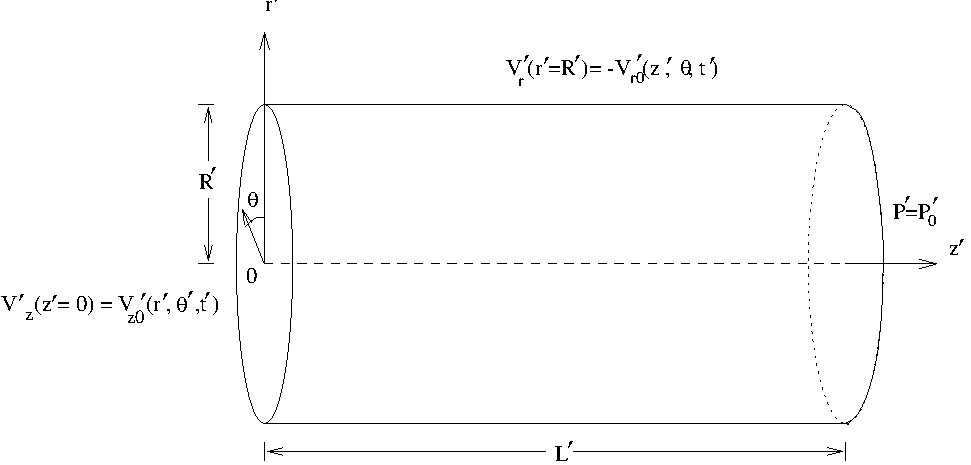
\includegraphics[width=100mm]{figs/cyl.pdf}
%     \end{center}
% \label{xfigDiagram}
% \end{figure}


% \begin{figure}[htbp]
%     \caption[Bitmap images]{
% 	The JPEG bitmap format is great for photos but
% 	crummy for diagrams (including drawings, graphs,
% 	charts) because it can't gracefully handle sharp edges.
% 	Note the same bitmap image below from a PNG file and
% 	from a JPG file; the latter shows characteristic
% 	``ringing'' at sharp edges -- including text!
% 	Seriously, magnify and look closely at the JPG's
% 	awful lines and edges.
% 	Vector-format PDF is the best for diagrams, but
% 	if you must use a bitmap image, let it be PNG.
% 	~ (Left: file {\it drawing.png}.
% 	Right: file {\it drawing.jpg}.)
% 	}
%     \begin{center}
% 	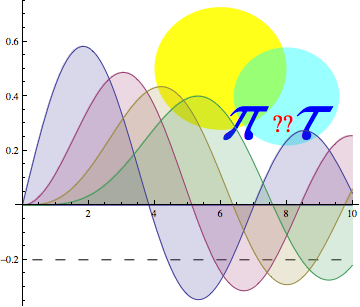
\includegraphics[width=70mm]{figs/drawing.png}
% 	${}^{}$ ~
% 	${}^{}$ ~
% 	${}^{}$
% 	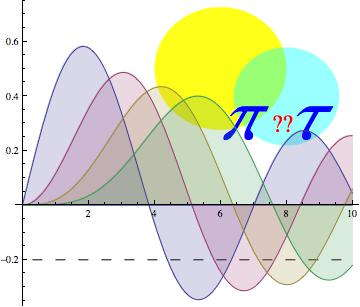
\includegraphics[width=70mm]{figs/drawing.jpg}
%     \end{center}
% \label{bitmapImages}
% \end{figure}



% \section{Lists in {\tt thesis} class}

% In {\tt thesis} class (for Colorado University),
% lists are defined so that nested lists will be
% numbered or marked appropriately.
% First, an itemized (non-enumerated) list
% prefaces each item with a bullet.
% Nested itemized list use asterisks,
% then dashes, then dots.
% These lists are typed between
% the \verb2\begin{itemize}2
% and \verb2\end{itemize}2
% commands.

% \begin{itemize}
%   \item{} This is ``itemized'' item A.
%   \item{} This is ``itemized'' item B.
%   \item{} This is ``itemized'' item C.
%   \begin{itemize}
%     \item{} This is ``itemized'' subitem A.
%     \begin{itemize}
%       \item{} This is ``itemized'' subsubitem A.
%       \begin{itemize}
%         \item{} This is ``itemized'' subsubsubitem A.
%       \end{itemize}
%       \item{} This is ``itemized'' subsubitem B.
%     \end{itemize}
%     \item{} This is ``itemized'' subitem B.
%   \end{itemize}
%   \item{} This is ``itemized'' item D.
% \end{itemize}

% Enumerated lists use the commands
% \verb2\begin{enumerate}2 and
% \verb2\end{enumerate}2,
% and nested enumerations appear like this.

% \begin{enumerate}
%   \item{} This is ``enumerated'' item A.
%   \item{} This is ``enumerated'' item B.
%   \item{} This is ``enumerated'' item C.
%   \begin{enumerate}
%     \item{} This is ``enumerated'' subitem A.
%     \begin{enumerate}
%       \item{} This is ``enumerated'' subsubitem A.
%       \begin{enumerate}
%         \item{} This is ``enumerated'' subsubsubitem A.
%       \end{enumerate}
%       \item{} This is ``enumerated'' subsubitem B.
%     \end{enumerate}
%     \item{} This is ``enumerated'' subitem B.
%   \end{enumerate}
%   \item{} This is ``enumerated'' item D.
% \end{enumerate}


% The work presented
% here\footnote{Footnotes are handled neatly by \LaTeX.}
% is an extension of Lao\cite{lao:thesis}
% and Lao et~al.\cite{lao:paper},
% fictional references that are in the bibliographic
% source file \verb9refs.bib9.

% \begin{table}[htb]
%     \caption[Example of a table with its own footnotes]{
% 	Here is an example of a table with its own footnotes.
% 	Don't use the $\backslash${\tt footnote} macro if you
% 	don't want the footnotes at the bottom of the page.
% 	Also, note that in a thesis the caption goes
% 	\emph{above} a table, unlike figures.
% 	}
%     \begin{center}
%     \begin{tabular}{||l|c|c|c|c||} \hline
% 	& $S$ & $P$ &   $Q^{\ast}$  & $D^{\dagger}$ \\	% footnote symbols!
% 	wave form & (kVA) & (kW) & (kVAr) & (kVAd) \\  \hline \hline
% 	Fig.  \ref{xfigDiagram}a  & 25.48 & 25.00 & -2.82 & 4.03 \\ \hline
% 	Fig.  \ref{xfigDiagram}b  & 25.11 & 18.02 & -9.75 & 14.52 \\ \hline
% 	Table \ref{pdftable}  & 24.98 & 22.26 & 9.19 & 6.64 \\ \hline
% 	Table \ref{powertable}  & 23.48 & 15.00 & 6.59 & 16.82 \\ \hline
% 	Fig.  \ref{pyramid}  & 24.64 & 22.81 & -0.44 & 9.3 \\ \hline
% 	\end{tabular}
%    \\ \rule{0mm}{5mm}
%    ${}^\ast$kVAr means reactive power.		% footnote symbol
% \\ ${}^\dagger$kVAd means distortion power.	% footnote symbol
% \end{center}
% \label{powertable}
% \end{table}


